\documentclass[simplex.tex]{subfiles}
% NO NEED TO INPUT PREAMBLES HERE
% packages are inherited; you can compile this on its own

\onlyinsubfile{
\title{NeuroData SIMPLEX Report: Subfile}
}

\begin{document}
\onlyinsubfile{
\maketitle
\thispagestyle{empty}

The following report documents the progress made by the labs of Randal~Burns and Joshua~T.~Vogelstein at Johns Hopkins University towards goals set by the DARPA SIMPLEX grant.

%%%% Table of Contents
\tableofcontents

%%%% Publications
\bibliographystyle{IEEEtran}
\begin{spacing}{0.5}
\section*{Publications, Presentations, and Talks}
%\vspace{-20pt}
\nocite{*}
{\footnotesize	\bibliography{simplex}}
\end{spacing}
%%%% End Publications
}


\subsection{FlashX}

\begin{figure}[h!]
\begin{cframed}
\centering
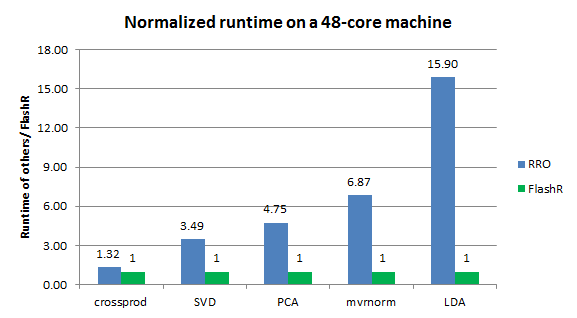
\includegraphics[width=0.5\textwidth]{../../figs/FlashR.vs.RRO.png}
\caption{
Normalized runtime of FlashR vs. Revolution R when executing R implementations
of machine learning primitives on a dataset with one million data points and
1000 features on a large parallel machine with
48 CPU cores. FlashR outperforms Revolution R in all computations. When
the computation gets more complex, the speed advantage of FlashR
over Revolution R gets larger.
}
\label{fig:flashr}
\end{cframed}
\end{figure}

After having efficient matrix operations in the past months, including sparse
matrix multiplication and various dense matrix operations, we integrate all
matrix operations in a single computation framework called FlashR, which
provides both high compatibility with R and efficiency. FlashR now overrides
about 70 R matrix functions in the R
\textit{base} package. As such, we can run existing R code with little
modification or no modification at all. For example, we ported a few R
implementations of machine learning algorithms in the \textit{MASS} package
with little modification. We compare the speed of FlashR against Revolution R,
which is also designed to parallelize and accelerate R code, on a large parallel
machine with 48 CPU cores (Figure \ref{fig:flashr}).
Even for the simple matrix operation such as \textit{crossprod}, FlashR
outperforms Revolution R. As the computation gets more complex, the advantage
of FlashR over Revolution R gets larger. When executing the LDA implementation
(Linear Discriminant Analysis) in the MASS package, FlashR outperforms Revolution R
by over an order of magnitude.


\end{document}
